%%%%%%%%%%%%%%%%%%%%%%%%%%%%%%%%%%%%%%%%%%%%%%%%%%%%%%%%%%%%%%%%%%%%%%%%%%%
%
% Template for a LaTex article.
%
%%%%%%%%%%%%%%%%%%%%%%%%%%%%%%%%%%%%%%%%%%%%%%%%%%%%%%%%%%%%%%%%%%%%%%%%%%%

\documentclass[12pt,a4paper]{article}
\usepackage{graphicx}
\usepackage[utf8]{inputenc}
\usepackage[T1]{fontenc}
\usepackage[english]{babel}
%\usepackage[spanish]{babel}
\usepackage{tikz}
\usetikzlibrary{arrows, arrows.meta}
\usepackage{framed}
\usepackage{float}
\usepackage{lipsum}
\usepackage[hidelinks]{hyperref}

%\hypersetup{linktocpage}

\usepackage{cprotect}

% AMS packages:
\usepackage{amsmath}
\usepackage{amsfonts}
\usepackage{amssymb}
\usepackage{amsthm}

% Pseudo code packages:
\usepackage{algpseudocode}
\usepackage{algorithm}

\usepackage{verbatim}
\newenvironment{metaverbatim}{\verbatim}{\endverbatim}

% Paragraphs and indentation control:
%\usepackage[skip, parfill]{parskip}
%\usepackage{parskip}
%\setlength{\parindent}{2em}
%\setlength{\parskip}{0.5em}
%\renewcommand{\baselinestretch}{1}



%\usepackage[firstpage]{draftwatermark} % [nostamp,firstpage]
%\SetWatermarkText{\textbf{DRAFT}}
%\SetWatermarkScale{4}
%\SetWatermarkColor[gray]{0.9}
%%\SetWatermarkLightness{0.95}
%%\SetWatermarkFontSize{5cm}
%%\SetWatermarkAngle{45}


% Theorems
%-----------------------------------------------------------------
\newtheorem{thm}{Theorem}[section]
\newtheorem{cor}[thm]{Corollary}
\newtheorem{lem}[thm]{Lemma}
\newtheorem{prop}[thm]{Proposition}
\theoremstyle{definition}
\newtheorem{defn}[thm]{Definition}
\theoremstyle{remark}
\newtheorem{rem}[thm]{Remark}

% Shortcuts.
% One can define new commands to shorten frequently used
% constructions. As an example, this defines the R and Z used
% for the real and integer numbers.
%-----------------------------------------------------------------
\def\RR{\mathbb{R}}
\def\ZZ{\mathbb{Z}}
\def\QQ{\mathbb{Q}}
\def\NN{\mathbb{N}}

% Similarly, one can define commands that take arguments. In this
% example we define a command for the absolute value.
% -----------------------------------------------------------------
\newcommand{\abs}[1]{\left\vert#1\right\vert}

% Tool box of new commands
\newcommand{\fparbox}[2][0.8\textwidth]{\fbox{\parbox{#1}{#2}}}

\newcommand{\ms}{\medskip}
\newcommand{\bs}{\bigskip}
\newcommand{\tbs}{\textbackslash}



% Operators
% New operators must defined as such to have them typeset
% correctly. As an example we define the Jacobian:
% -----------------------------------------------------------------
\DeclareMathOperator{\Jac}{Jac}
% This makes the same as \DeclareMathOperator{\Jac}{Jac}
% \newcommand{\Jac}{\operatorname{Jac}}
\DeclareMathOperator{\Ker}{Ker}
\DeclareMathOperator{\Max}{Max}
\DeclareMathOperator{\End}{End}



%-----------------------------------------------------------------
\title{Template for a \LaTeX\ article}
\author{Angela Menéndez\\
  \small A-level, Year 12D\\
  \small TEMS\\
  \small Madrid
}



\begin{document}

\maketitle

\begin{abstract}
This is a simple template for an article written in \LaTeX, with a few useful examples as introduction to pdflatex environment.

Since we are in the abstract, it is worth to mention that the Abstract will be open and close like this:
\begin{verbatim}
\begin{abstract}
    Abstact text here ...
\end{abstract}
\end{verbatim}

It is not recommended to use the command
\texttt{\textbackslash abstract},
\begin{verbatim}
\abstract{
    Abstact text here ...
}
\end{verbatim}

This second way to introduce the abstract will make the control of paragraphs indentation and spacing more tedious,
 

\end{abstract}

\newpage
\tableofcontents

\newpage
\section{Introduction to boxes and minipages}

\subsection{Boxing Paragraphs}

\begin{verbatim}
\fbox{\parbox{1\textwidth}{
\lipsum[1]
}
\end{verbatim}
\bigskip 

\noindent
\fbox{\parbox{1\textwidth}{
\lipsum[1]}}
\bigskip 

\begin{verbatim}
\fbox{\parbox{0.8\textwidth}{
\lipsum[2]
}
\end{verbatim}
\bigskip 

\noindent
\fbox{\parbox{0.8\textwidth}{\lipsum[2]}}
\bigskip 

\newpage
\begin{verbatim}
\begin{center}
\fbox{\parbox{0.8\textwidth}{
    \lipsum[3-5]
}
\end{center}
\end{verbatim}
\bigskip 

\noindent
\begin{center}
\fbox{\parbox{0.8\textwidth}{\lipsum[3-5]}}
\end{center}
 
\begin{verbatim}
\fbox{
\begin{minipage}[c]{0.7\textwidth}
  \lipsum[16]
\end{minipage}
}
\end{verbatim}
\bigskip 

\noindent
\fbox{
\begin{minipage}[c]{0.7\textwidth}
  \lipsum[16]
\end{minipage}
}
\bigskip 

\begin{verbatim}
\begin{center}
\fbox{
\begin{minipage}[c]{0.7\textwidth}
  \lipsum[16]
\end{minipage}
}
\end{center}
\end{verbatim}
\bigskip 

\begin{center}
\fbox{
\begin{minipage}[c]{0.7\textwidth}
  \lipsum[16]
\end{minipage}
}
\end{center}
\bigskip 



\begin{verbatim}
\fbox{\parbox{0.8\textwidth}{
    The quick brown fox jumps right over the lazy dog
}}
\end{verbatim}
\bigskip 

\fbox{\parbox{0.8\textwidth}{
    The quick brown fox jumps right over the lazy dog
}}


\subsection{Some paragraphs generated with \texttt{\textbackslash usepackage\{lipsum\} }}

\begin{verbatim}
\lipsum[1-7]
\end{verbatim}
\hrule \bigskip 

\lipsum[1-7]

\newpage 
\cprotect\subsection{Include\verb-\verb- anywhere! (Boxing verbatim)}

The \texttt{cprotect} package attempts to do something that should be impossible: it allows you
to put verbatim in footnotes, section titles, . . . in a straightforward way. The section above was typeset using

\begin{verbatim}
\cprotect\subsection{Include\verb-\verb- anywhere! (Boxing verbatim)}
\end{verbatim}

The normal way for boxing a paragraph or a piece of text is like follows.
\bs

\begin{minipage}{0.45\textwidth}
\begin{verbatim}
\fbox {
    \parbox{0.9\linewidth}{
    This is some text!
    Blah blah blah...
    }
}
\end{verbatim}
\end{minipage}
\hfill\vline\hfill
\begin{minipage}[c]{0.3\textwidth}
\fbox{
    \parbox{0.9\linewidth}{
    This is some text! Blah blah blah...
    }}
\end{minipage}
\bs

It gets more complicated when trying to box a piece of text with a verbatim environment on it.
\bigskip 

\begin{minipage}{0.55\textwidth}
\begin{verbatim}
\fbox{
\parbox{0.9\linewidth}{
This some normal text ...
\begin{verbatim}
  This is some verbatim text ...
\-end{verbatim}
And this is even more normal text.
}}
\end{verbatim}
\end{minipage}
\vline\hfill
\begin{minipage}[c]{0.35\textwidth}
\begin{verbatim}
Error:
! Argument of \@xverbatim has
an extra }.<inserted text>\par }
\end{verbatim}
\end{minipage}
\bigskip

To be able to boxed a text with \texttt{verbatim} on it you have
use the package \texttt{\tbs usepackage\{cprotect\}}, and type something like: \bs

\begin{minipage}{0.55\textwidth}
\noindent
\texttt{\tbs cprotect\tbs fbox\{\\
\tbs begin\{minipage\}\{0.8\tbs textwidth\}\\
This some normal text and\\
 \tbs begin\{verbatim\}\\
 \hphantom{ } This is some verbatim text ...\\
 \tbs end\{verbatim\}\\
And this is even more normal text.\\
\tbs end\{minipage\}\\
\}}
\end{minipage}
\vline\hspace{0.5em}
\cprotect\fbox{
\begin{minipage}[c]{0.47\textwidth}
This some normal text and
\begin{verbatim}
This is some verbatim text ...
\end{verbatim}
And this is even more normal text.
\end{minipage}
}



\begin{center}
\begin{minipage}[c]{0.8 \textwidth}
The above text was not easy to produce, to \texttt{verbatim} an \texttt{\tbs end\{verbatim\}} is not strait forward.
\begin{verbatim}
\noindent
\texttt{\tbs cprotect\tbs fbox\{\\
\tbs begin\{minipage\}\{0.8\tbs textwidth\}\\
This some normal text and\\
 \tbs begin\{verbatim\}\\
 \hphantom{ } This is some verbatim text ...\\
 \tbs end\{verbatim\}\\
And this is even more normal text.\\
\tbs end\{minipage\}\\
\}
\end{verbatim}
\end{minipage}
\end{center}


% This a another way to produce the above paragraph,
% much easier but with en error on \end{verbatim}
% as of today I haven't find a better way to verbatim a \end{verbatim}

%\begin{verbatim}
%\cprotect\fbox{
%\begin{minipage}{0.8\textwidth}
%This some normal text and 
%\begin{verbatim}
% This is some verbatim text ...
%\*end{verbatim}
%And this is even more normal text.
%\end{minipage}
%}
%\end{verbatim}



\subsection{Boxing math equations}
For boxing equation \texttt{\textbackslash boxed{}} has to be used.
\bigskip 

\begin{minipage}{0.35\textwidth}
\begin{verbatim}
\begin{equation}
 \boxed{x^2+y^2 = z^2}
\end{equation}
\end{verbatim}
\end{minipage}
\hfill\vline\hfill
\begin{minipage}[c]{0.35\textwidth}
\begin{equation}
 \boxed{x^2+y^2 = z^2}
\end{equation}
\end{minipage}\\ \\

\noindent
\verb|\boxed{}| can be used as inline maths just in the middle of normal paragraph text.\\

\begin{minipage}{0.45\textwidth}
\begin{verbatim}
The next equation 
\boxed{x^2+y^2 = z^2} 
represents the 3D sphere.
\end{verbatim}
\end{minipage}
\hfill\vline\hfill
\begin{minipage}[c]{0.45\textwidth}
The next equation \boxed{x^2+y^2 = z^2} represents the 3D sphere.
\end{minipage}\\ \\



\section{Some maths typing examples}\label{sec:maths_examples}

Here goes the text of this first section.


\begin{equation}\label{eq:area}
  S = \pi r^2
\end{equation}
\[S_n = \sum_{n=1}^{\infty} \frac{1}{n^3} + \sum_{n=1}^{\infty} \frac{1}{n^3}\] 

One can refer to equations like this: see equation (\ref{eq:area}). One can also refer to sections in the same way: see section \ref{sec:pictures_graphs}. Or
to the bibliography like this: \cite{Cd94} just typing \verb|\cite{Cd94}|.

One can refer to equations like this: see equation (\ref{eq:area}). One can also
refer to sections in the same way: see section \ref{sec:pictures_graphs}. Or
to the bibliography like this: \cite{Cd94}.

More text. Claro 
\noindent
\[\RR\ \text{is the set of real numbers}\]
\[\QQ\ \text{is the set of rational numbers}\]
\[\ZZ\ \text{is the set of integer numbers}\]
\[\NN\ \text{is the set of natual numbers}\]



\subsection{\AmS-\LaTeX \texttt{ amsmaths} package}\label{sec:nothing}
\begin{verbatim}
\usepackage{amsmath, amsthm, amsfonts}
\end{verbatim}

In this section a few examples of the use of 
\verb|\DeclareMathOperator| will we put in practice.

In the preamble of the document the Math Operator have to be defined 
\begin{verbatim}
\DeclareMathOperator{\Jac}{Jac}
% This makes the same as \DeclareMathOperator{\Jac}{Jac}
% \newcommand{\Jac}{\operatorname{Jac}}
\DeclareMathOperator{\Ker}{Ker}
\DeclareMathOperator{\Max}{Max}
\DeclareMathOperator{\End}{End}
\end{verbatim}

\bigskip
\begin{minipage}[t]{0.55\textwidth}
\textbf{The \LaTeX \ code:}
\begin{verbatim}
\begin{displaymath}
 \Max_{x \in A} f(x) \quad \End_R V 
\end{displaymath}
\end{verbatim}
\end{minipage}
\vline\hfill
\begin{minipage}[t]{0.35\textwidth}
\textbf{Will produces the next math formula:}
\begin{displaymath}
 \Max_{x \in A} f(x) \quad \End_R V 
\end{displaymath}
\end{minipage}


\section{Pseudo code algorithms}\label{sec:pseudo_code}

This is my first algorithm with \LaTeX

\begin{algorithmic}[1]
\State $i \gets 10$
\If{$i\geq 5$} 
    \State $i \gets i-1$
\Else
    \If{$i\leq 3$}
        \State $i \gets i+2$
    \EndIf
\EndIf 
\end{algorithmic}

\bigskip 
And next is the second
\begin{algorithmic}
\Require $n \geq 0$
\Ensure $y = x^n$
\State $y \gets 1$
\State $X \gets x$
\State $N \gets n$
\While{$N \neq 0$}
\If{$N$ is even}
    \State $X \gets X \times X$
    \State $N \gets \frac{N}{2}$  \Comment{This is a comment}
\ElsIf{$N$ is odd}
    \State $y \gets y \times X$
    \State $N \gets N - 1$
\EndIf
\EndWhile
\end{algorithmic}



The complete pseudo code with titles:

\begin{algorithm}
\caption{An algorithm with caption}\label{alg:cap}
\begin{algorithmic}[1]
\Require $n \geq 0$
\Ensure $y = x^n$
\State $y \gets 1$
\State $X \gets x$
\State $N \gets n$
\While{$N \neq 0$}
\If{$N$ is even}
    \State $X \gets X \times X$
    \State $N \gets \frac{N}{2}$  \Comment{This is a comment}
\ElsIf{$N$ is odd}
    \State $y \gets y \times X$
    \State $N \gets N - 1$
\EndIf
\EndWhile
\end{algorithmic}
\end{algorithm}



\section{Pictures and graphs}\label{sec:pictures_graphs}

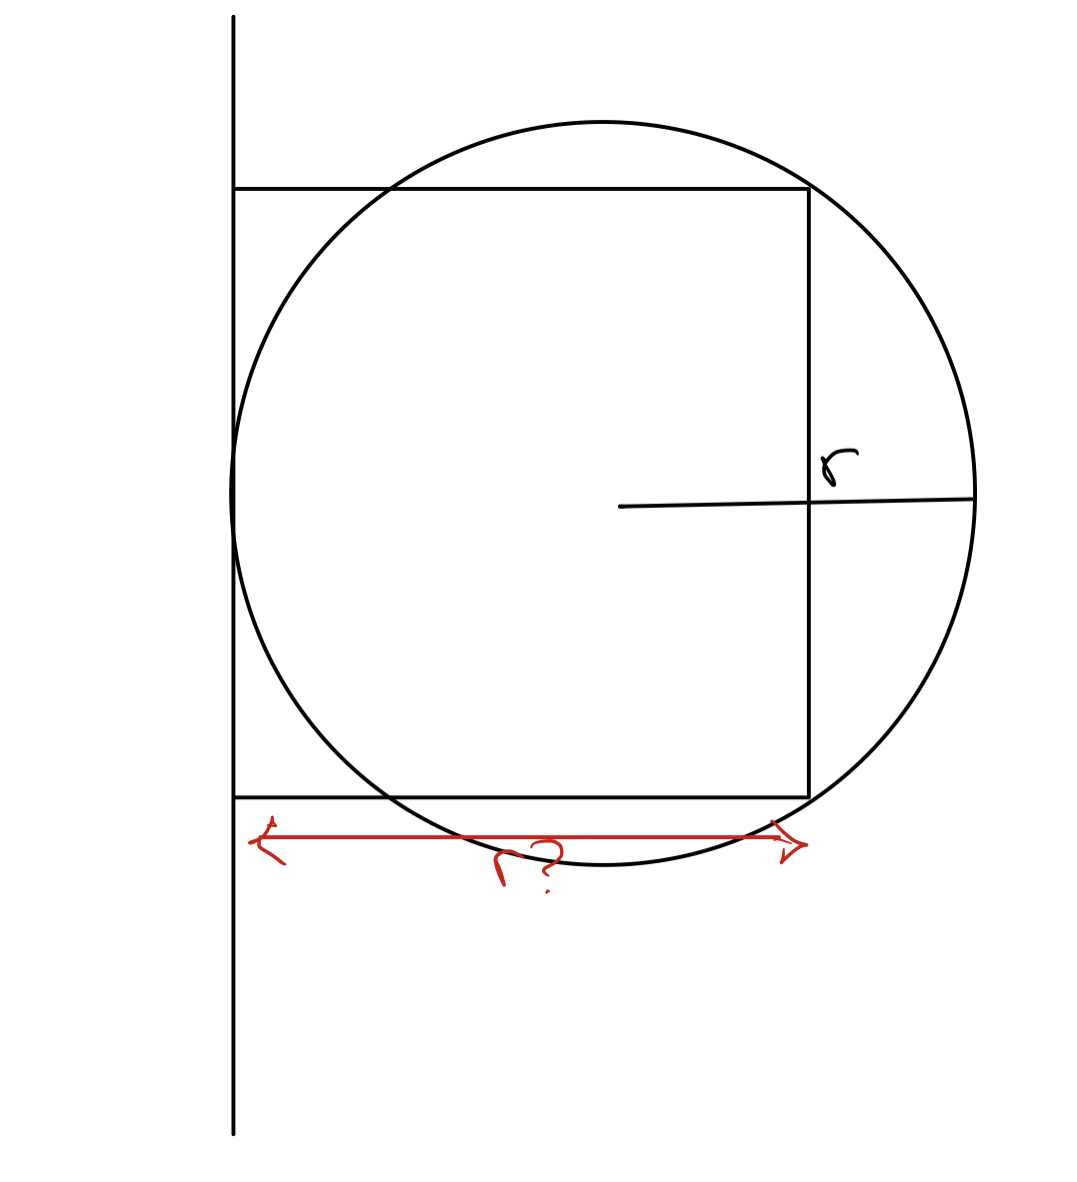
\includegraphics[width=0.6\textwidth]{./figs/radius_scure.jpg}

\subsection{Version with TikZ graphics package}
Know the version with TikZ graphics package \verb|\usepackage{tikz}| and \newline \verb|\usetikzlibrary{arrows, arrows.meta}| 

\begin{center}
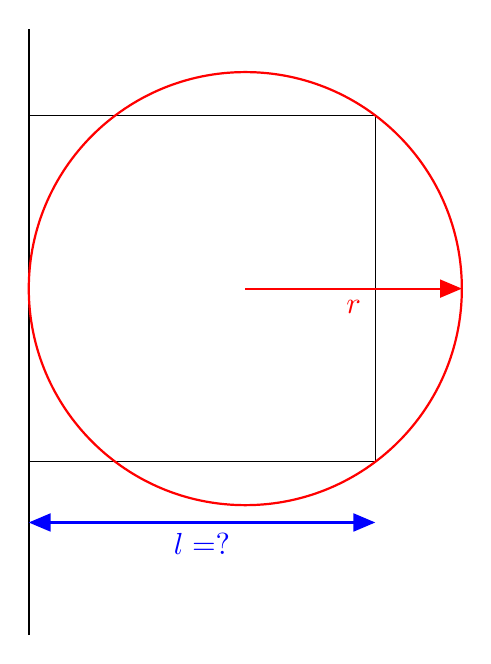
\begin{tikzpicture}[scale=1.1, transform shape]
\draw (0,0) -- (4,0) -- (4,4) -- (0,4) -- cycle;
\draw[thick] (0,-2) -- (0,5);
\draw[red,thick] (2.5,2) circle (2.5cm);
\draw[>=triangle 45,->,red,thick] (2.5,2) -- (5,2) node[midway,below] {$r$};
\draw[>=triangle 45,<->,blue,thick] (0,-0.7) -- (4,-0.7) node[midway,below] {$l=?$};
\end{tikzpicture}
\end{center}


\subsubsection{Subsubsection}\label{sec:nothing2}

More text \cite{Someone2000}


\includegraphics[width=0.8\textwidth]{./figs/latex_logo.png}


\section{LaTeX Graphics using TikZ}

\bigskip 
\begin{center}
\begin{tikzpicture}
\draw (0,0) -- (8,0) -- (8,8) -- (0,8) -- (0,0);
\end{tikzpicture}
\end{center}


\bigskip 
\begin{tikzpicture}
\draw (0,0) -- (8,0) -- (8,8) -- cycle;
\draw (0,0) parabola (-4,8);
\end{tikzpicture}

\bigskip 
\begin{tikzpicture}
\draw (0,0) .. controls (0,10) and (10,0) .. (10,10);
\end{tikzpicture}


\bigskip 
\begin{tikzpicture}
\draw (0,0) -- (1,0) -- (1,1) -- (0,1) -- (0,0);
\draw[red,thick,dashed] (3,3) circle (4cm);
\end{tikzpicture}

\bigskip 
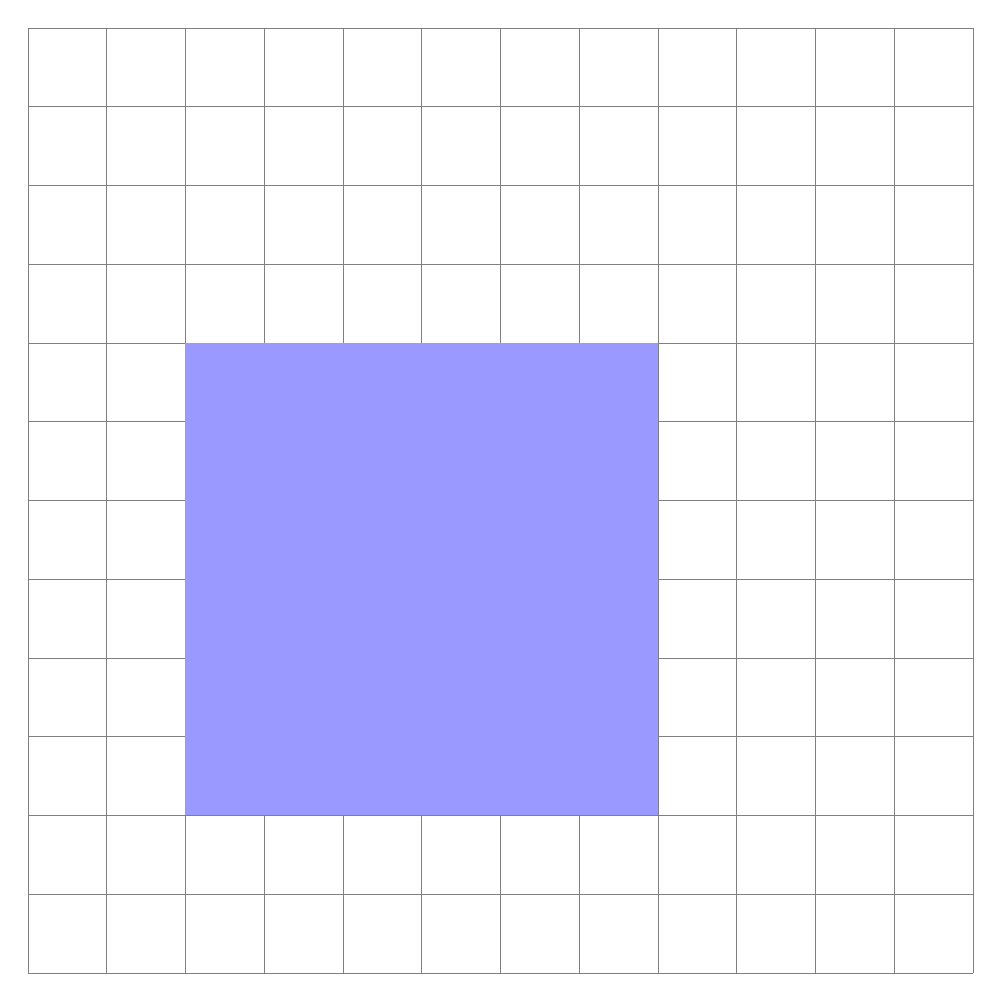
\begin{tikzpicture}
\draw[step=1cm,gray,very thin] (-2,-2) grid (10,10);
\fill[blue!40!white] (0,0) rectangle (6,6);
\end{tikzpicture}

\bigskip 
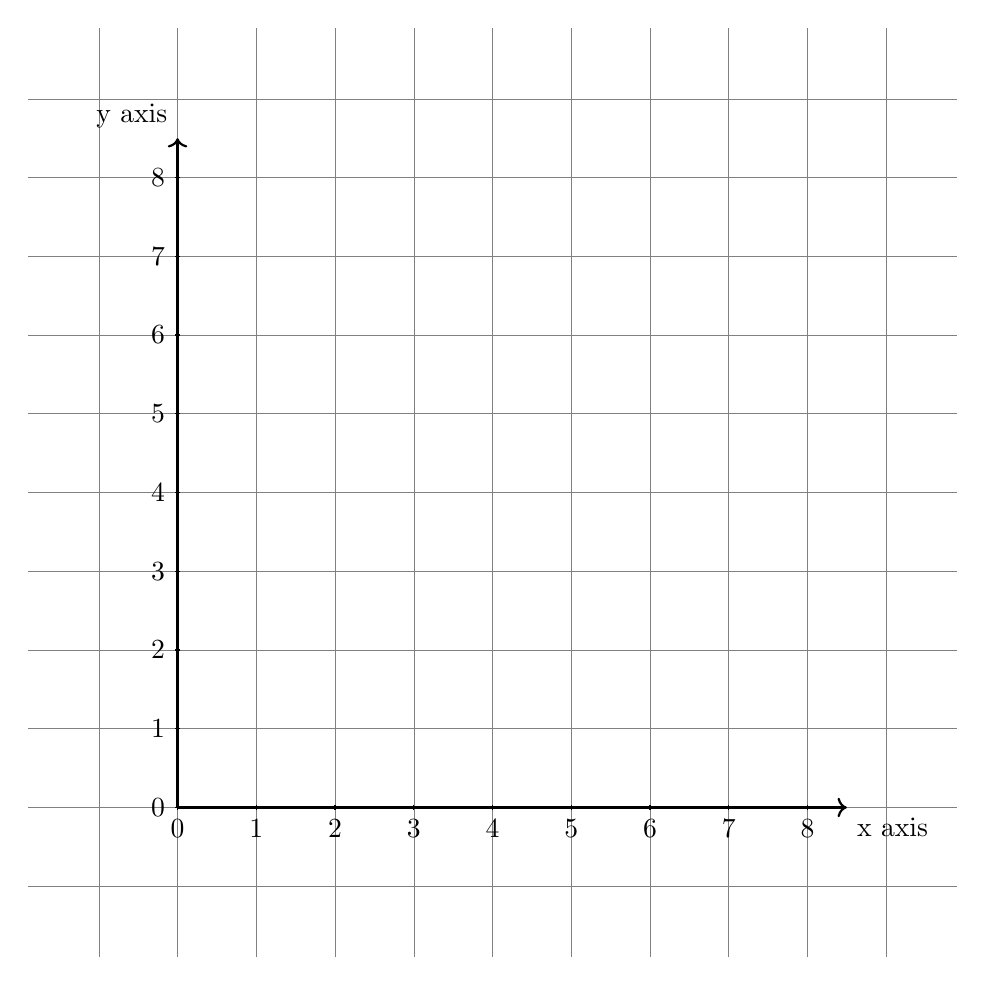
\begin{tikzpicture}
\draw[step=1cm,gray,very thin] (-1.9,-1.9) grid (9.9,9.9);
\draw[thick,->] (0,0) -- (8.5,0) node[anchor=north west] {x axis};
\draw[thick,->] (0,0) -- (0,8.5) node[anchor=south east] {y axis};

\foreach \x in {0,1,2,3,4,5,6,7,8}
   \draw (\x cm,1pt) -- (\x cm,-1pt) node[anchor=north] {$\x$};
\foreach \y in {0,1,2,3,4,5,6,7,8}
    \draw (1pt,\y cm) -- (-1pt,\y cm) node[anchor=east] {$\y$};
    
\end{tikzpicture}

\bigskip 
\begin{tikzpicture}
\draw[red,thick] (0,0) circle (0.1cm);
\draw (0,0) arc (270:0:4cm);
\end{tikzpicture}

\noindent
Nodes connected with lines and text in the line.

\bigskip
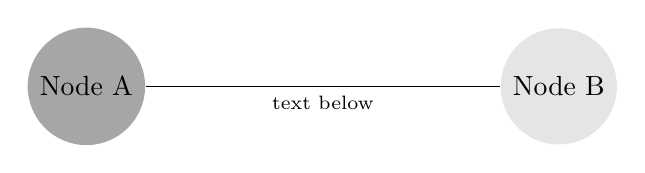
\begin{tikzpicture}[scale=1,auto=center]
  \node[circle,fill=gray!70] (n1) at (2,8) {Node A};
  \node[circle,fill=gray!20] (n2) at (8,8) {Node B};
  \foreach \from/\to in {n1/n2}
  \draw (\from) -- (\to) node[draw=none,fill=none,font=\scriptsize,midway,below] {text below};
\end{tikzpicture}

\bigskip
\begin{center}
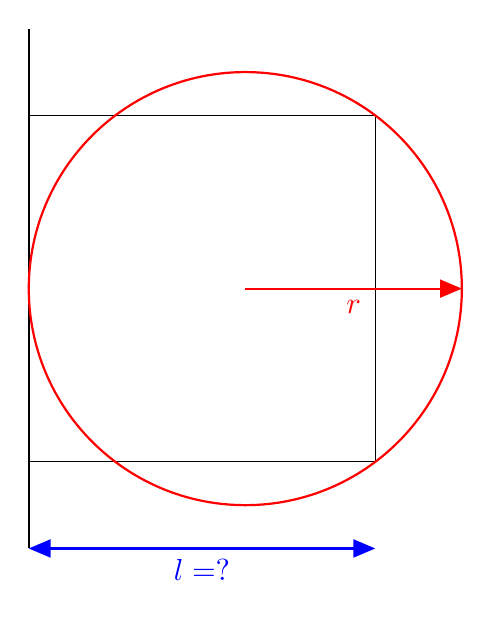
\begin{tikzpicture}[scale=1.1, transform shape]
\draw (0,0) -- (4,0) -- (4,4) -- (0,4) -- cycle;
\draw[thick] (0,-1) -- (0,5);
\draw[red,thick] (2.5,2) circle (2.5cm);
\draw[>=triangle 45,->,red,thick] (2.5,2) -- (5,2) node[midway,below] {$r$};
\draw[>=triangle 45,<->,blue,thick] (0,-1) -- (4,-1) node[midway,below] {$l=?$};
\end{tikzpicture}
\end{center}


\section{Paragraphs formatting}\label{sec:par_formatting}
\begin{verbatim}
\usepackage{parskip}
%\usepackage[skip, parfill]{parskip}
\setlength{\parindent}{4em}
\setlength{\parskip}{1em}
\renewcommand{\baselinestretch}{1}
\end{verbatim}

%\begin{figure}[hbtp]
\begin{figure}[H]
\centering
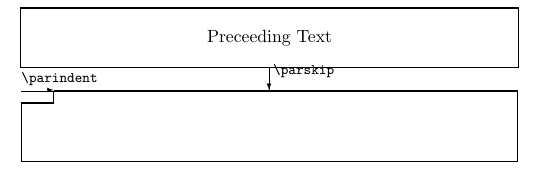
\includegraphics[scale=0.7]{./figs/Paragraph-layout.png}
\caption{Paragraph indentation and spacing}
\end{figure}

\subsection{Paragraph indentation}\label{sec:par_indentation}

\lipsum[1]

\setlength{\leftskip}{2cm}
\lipsum[2]

\setlength{\leftskip}{0pt}
\lipsum[3]


\newenvironment{myindentpar}[1]%
{\begin{list}{}
         {\setlength{\leftmargin}{#1}}
         \item[]
}
{\end{list}}

\begin{myindentpar}{5em}
\lipsum[4]
\end{myindentpar}

\lipsum[1]
\newpage
\subsubsection{Indenting paragraphs with \texttt{itemize}}
Lorem ipsum dolor sit amet, consectetuer adipiscing elit. Ut purus elit, vestibulum ut, placerat ac, adipiscing vitae, felis. Curabitur dictum gravida mauris. Nam arcu libero, nonummy eget, consectetuer id, vulputate a,magna.
\begin{itemize}
\item[]
	Fusce mauris. Vestibulum luctus nibh at lectus. Sed bibendum, nulla a faucibus semper, leo velit ultricies tellus, ac venenatis arcu wisi vel nisl. Vestibulum diam. Aliquam pellentesque, augue quis sagittis posuere, turpis lacus congue quam, in hendrerit risus eros eget felis.
\begin{itemize}
\item[]
Maecenas eget erat in sapien mattis porttitor.
Vestibulum porttitor. Nulla facilisi. Sed a turpis eu lacus commodo
facilisis. Morbi fringilla, wisi in dignissim interdum, justo lectus
sagittis dui, et vehicula libero dui cursus dui. Mauris tempor ligula
sed lacus. Duis cursus enim ut augue. Cras ac magna. Cras nulla.
Nulla egestas. Curabitur a leo. Quisque egestas wisi eget nunc.
Nam feugiat lacus vel est. Curabitur consectetuer.
\end{itemize} 
\end{itemize}



\section{metaverbatim}


\begin{metaverbatim}
\begin{verbatim}
  This is a verbatim block.
\end{verbatim}
\end{metaverbatim}

\hrule
\begin{metaverbatim}
\documentclass{article}
\usepackage{verbatim}
\newenvironment{metaverbatim}{\verbatim}{\endverbatim}

\begin{document}
\begin{metaverbatim}
\begin{verbatim}
  This is a verbatim block.
\end{verbatim}
\end{metaverbatim}
\end{document}
\end{metaverbatim}




\newpage
% Bibliography
%-----------------------------------------------------------------
\begin{thebibliography}{99}

\bibitem{Cd94} 
	Author,
	\emph{Title}
	\newblock{Journal/Editor, (year)}


\bibitem{Author1990}
    A.~Author.
    \newblock {\em Handbook of Everything}.
    \newblock Some Press, 1990.

  \bibitem{Someone2000}
    S.~Someone.
    \newblock On this and that.
    \newblock {\em Journal of This and That}, 2(1):50--100,
    2000.
\end{thebibliography}


\end{document}
